\documentclass[11pt]{article}
\usepackage[letterpaper,margin=0.86in]{geometry}
\usepackage{amsmath,amssymb,amsthm,mathtools,graphicx,microtype,xcolor}
\usepackage[colorlinks=true,linkcolor=blue!55!black,citecolor=blue!55!black,urlcolor=blue!55!black]{hyperref}

\newtheorem{theorem}{Theorem}
\newtheorem{lemma}[theorem]{Lemma}
\newtheorem{corollary}[theorem]{Corollary}
\newtheorem{remark}[theorem]{Remark}
\newcommand{\R}{\mathbb R}
\newcommand{\G}{\Gamma}
\newcommand{\nuG}{\boldsymbol\nu}
\newcommand{\BG}{\mathbf B}
\newcommand{\PG}{\mathbf P}
\newcommand{\nG}{\nabla_{\!\G}}
\newcommand{\nM}{\nabla_{\!M}}
\newcommand{\divG}{\operatorname{div}_{\!\G}}
\newcommand{\Lp}[1]{L^{#1}(\G)}
\newcommand{\Wp}[1]{W^{1,#1}(\G)}
\newcommand{\Wtp}[1]{\mathbf W^{1,#1}_t(\G)}

\title{The covariant-gradient Poincar\'e inequality on closed $C^{1,1}$ hypersurfaces}
\author{Candidate full answer to the open question in arXiv:2508.11109}
\date{11 August 2026}

\begin{document}
\maketitle

\noindent\fbox{\parbox{0.95\linewidth}{\textbf{Status.}
Candidate full affirmative result, likely valid, requiring human review.
For every compact connected embedded $C^{1,1}$ hypersurface of intrinsic
dimension at least two, the covariant gradient is injective on tangential
$W^{1,p}$ fields and satisfies the full Poincar\'e estimate, for every
$1<p<\infty$.  This answers the exact regularity question following Lemma
3.2 of the source and lowers its weak $L^2$ Bochner--Laplace theory to
$C^{1,1}$.}}

\section{The source question and the answer}

Let $\G\subset\R^{d+1}$ be a compact connected embedded hypersurface without
boundary, where $d\ge2$.  The source proves, under $\G\in C^2$, that the
covariant gradient $\nG$ is injective on tangential fields and consequently
that
\begin{equation}\label{eq:source-poincare}
 \|v\|_{W^{1,p}(\G)}\le C\|\nG v\|_{L^p(\G)},
 \qquad v\in\Wtp p.
\end{equation}
It then explicitly asks whether $C^2$ can be replaced by $C^{1,1}$.

\begin{figure}[ht]
\centering
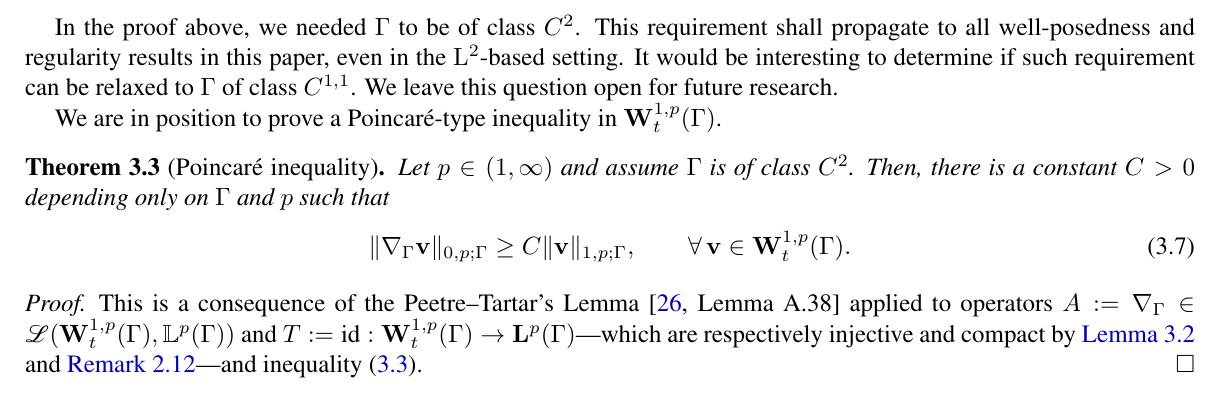
\includegraphics[width=0.96\linewidth]{figures/open_question_and_poincare.png}
\caption{The open $C^{1,1}$ question and the ensuing Poincar\'e theorem in
the current source PDF~\cite[p.~14]{BNS}.}
\end{figure}

The obstruction in the printed proof is precise.  For a $C^2$ hypersurface,
continuity of the shape operator gives a nonempty open set on which the
Gauss--Kronecker curvature does not vanish.  For $C^{1,1}$, the shape
operator exists only almost everywhere, so that topological step cannot be
copied.  The replacement is the area formula for the Lipschitz Gauss map:
it produces a \emph{positive-measure} set on which the shape operator is
invertible.  A low-regularity curvature compatibility argument is then
enough.

\begin{theorem}[Affirmative answer]\label{thm:main}
Let $d\ge2$, $1<p<\infty$, and let $\G\subset\R^{d+1}$ be a compact,
connected, embedded $C^{1,1}$ hypersurface without boundary.  If
$v\in\Wtp p$ and $\nG v=0$ almost everywhere, then $v=0$ almost everywhere.
Moreover, there is a constant $C=C(\G,p)$ such that
\begin{equation}\label{eq:main-poincare}
 \|v\|_{W^{1,p}(\G)}\le C\|\nG v\|_{L^p(\G)}
 \qquad\text{for every }v\in\Wtp p.
\end{equation}
\end{theorem}

\section{Three low-regularity lemmas}

Write $\nuG$ for the outward unit normal, $\PG=I-\nuG\otimes\nuG$, and
$\BG=\nM\nuG$.  On a $C^{1,1}$ hypersurface, $\nuG$ is Lipschitz and
$\BG\in L^\infty$; $\BG$ is self-adjoint on the tangent space almost
everywhere.

\begin{lemma}[The Gauss map has nonsingular differential on a set of positive
measure]\label{lem:gauss-map}
The set
\[
 E:=\{x\in\G:\det(\BG(x)|_{T_x\G})\ne0\}
\]
has positive $d$-dimensional surface measure.
\end{lemma}

\begin{proof}
The map $\nuG:\G\to S^d$ is Lipschitz.  It is onto.  Indeed, fix
$\omega\in S^d$ and maximize $x\mapsto x\cdot\omega$ on $\G$.  At a
maximizer, $\omega$ is normal to $\G$.  Jordan--Brouwer separation makes
$\G$ the boundary of its bounded complementary component, which lies in the
supporting halfspace $x\cdot\omega\le\max_{\G}y\cdot\omega$; hence the
outward normal there is $\omega$.

Apply the area formula to the Lipschitz map $\nuG$ between the two
$d$-manifolds.  If $N(\nuG,\omega)$ is its multiplicity, then
\begin{equation}\label{eq:area}
 \int_{\G}J_{\G}\nuG\,d\mathcal H^d
 =\int_{S^d}N(\nuG,\omega)\,d\mathcal H^d(\omega)
 \ge \mathcal H^d(S^d).
\end{equation}
Rademacher's theorem and the definition of the shape operator give
$J_{\G}\nuG=|\det\BG|$ almost everywhere.  The integral in
\eqref{eq:area} is positive, so $E$ has positive measure.
\end{proof}

\begin{lemma}[A weakly parallel field is Lipschitz and has constant
length]\label{lem:bootstrap}
If $v\in\Wtp p$ and $\nG v=0$ almost everywhere, then
$v\in W^{1,\infty}(\G;\R^{d+1})$ and $|v|$ is constant almost everywhere
on $\G$.
\end{lemma}

\begin{proof}
Work in a $C^{1,1}$ chart.  Differentiating $v\cdot\nuG=0$ weakly and using
that the tangential part of every first derivative of $v$ vanishes yields
\begin{equation}\label{eq:first-order}
 \partial_i v=-(v\cdot\partial_i\nuG)\nuG=A_i v
 \qquad\text{a.e.},
\end{equation}
where $A_i\in L^\infty$.  If the current integrability exponent $q$ is below
$d$, Sobolev embedding first gives $v\in L^{q^*}$, where
$q^*=dq/(d-q)$, and \eqref{eq:first-order} then gives
$v\in W^{1,q^*}$.  Iteration reaches an exponent at least $d$ in finitely
many steps.  At the endpoint $q=d$, use $W^{1,d}\hookrightarrow L^r$ for
every finite $r$; once $q>d$, Morrey gives $v\in L^\infty$.  Equation
\eqref{eq:first-order} finally gives $v\in W^{1,\infty}$.

Now
\[
 \partial_i|v|^2=2v\cdot\partial_i v
 =-2(v\cdot\partial_i\nuG)(v\cdot\nuG)=0
\]
almost everywhere.  A Sobolev function with zero weak gradient is constant
on the connected manifold $\G$.
\end{proof}

The next lemma records the only compatibility fact whose regularity needs
care.  It is the $C^{1,1}$ version of ``a parallel field is annihilated by
curvature.''

\begin{lemma}[Weak Gauss compatibility]\label{lem:weak-gauss}
Under the hypotheses of Lemma~\ref{lem:bootstrap}, for almost every
$x\in\G$ and all $X,Y\in T_x\G$,
\begin{equation}\label{eq:gauss-compatibility}
 (v\cdot\BG Y)\BG X-(v\cdot\BG X)\BG Y=0.
\end{equation}
\end{lemma}

\begin{proof}
Choose a local $C^{1,1}$ parametrization $F:U\to\G$.  The induced metric is
$W^{1,\infty}$, its Christoffel matrices $\Gamma_i$ belong to
$L^\infty$, and the coordinate vector $V$ of $v$ belongs to
$W^{1,\infty}$ by Lemma~\ref{lem:bootstrap}.  Parallelity says
\begin{equation}\label{eq:parallel-coordinates}
 \partial_iV+\Gamma_iV=0\qquad\text{a.e. on }U.
\end{equation}
Commuting the two distributional first-order operators in
\eqref{eq:parallel-coordinates} gives
\begin{equation}\label{eq:curv-kills}
 \bigl(\partial_i\Gamma_j-\partial_j\Gamma_i
       +\Gamma_i\Gamma_j-\Gamma_j\Gamma_i\bigr)V=0
 \qquad\text{in }\mathcal D'(U).
\end{equation}
This calculation is legitimate at exactly this regularity: products of an
$L^\infty$ coefficient with $V$ or $\partial V$ are integrable, and a term
such as $(\partial_i\Gamma_j)V$ is defined by the Leibniz identity
$\partial_i(\Gamma_jV)-\Gamma_j\partial_iV$.

For completeness, the Gauss identity also survives at this regularity.
If $g_{ij}=\partial_iF\cdot\partial_jF$ and
$h_{ij}=\partial_{ij}F\cdot\nuG$, then the coordinate expansion of the
distributional curvature gives
\begin{equation}\label{eq:weak-gauss-coordinate}
 \langle R(\partial_i,\partial_j)\partial_k,\partial_l\rangle
 =h_{il}h_{jk}-h_{ik}h_{jl}\qquad\text{a.e.}
\end{equation}
The apparent third derivatives of $F$ cancel because distributional mixed
partials commute; every remaining term is a product of $L^\infty$ second
derivatives.  Thus the curvature distribution in \eqref{eq:curv-kills} is
represented by the $L^\infty$ tensor in
\eqref{eq:weak-gauss-coordinate}.  Consequently $R(X,Y)v=0$ almost
everywhere.  Rewriting \eqref{eq:weak-gauss-coordinate} with
$h(X,Y)=\langle\BG X,Y\rangle$ yields exactly
\eqref{eq:gauss-compatibility}.
\end{proof}

\section{Proof of the theorem}

\begin{proof}[Proof of Theorem~\ref{thm:main}]
Let $v\in\Wtp p$ and $\nG v=0$.  At almost every point $x\in E$ from
Lemma~\ref{lem:gauss-map}, diagonalize the self-adjoint shape operator:
$\BG e_i=\kappa_i e_i$, where all $\kappa_i\ne0$.  Write
$v=\sum_i v_i e_i$.  Lemma~\ref{lem:weak-gauss}, with $X=e_i$ and
$Y=e_j$, gives for $i\ne j$
\begin{equation}\label{eq:diagonal}
 0=\kappa_i\kappa_j(v_j e_i-v_i e_j).
\end{equation}
Because $d\ge2$, for every index one may choose a different index in
\eqref{eq:diagonal}; hence every $v_i=0$.  Thus $v=0$ almost everywhere on
the positive-measure set $E$.  Lemma~\ref{lem:bootstrap} says that $|v|$ is
constant, so that constant is zero.  This proves injectivity.

It remains to prove the estimate.  The a.e. tangential derivative identity
\begin{equation}\label{eq:norm-comparison}
 \nM v=\nG v-\nuG v^T\BG
\end{equation}
and $\BG\in L^\infty$ give
\begin{equation}\label{eq:weak-poincare}
 \|v\|_{W^{1,p}(\G)}
 \le C_0\bigl(\|\nG v\|_{L^p(\G)}+\|v\|_{L^p(\G)}\bigr).
\end{equation}
If \eqref{eq:main-poincare} failed, there would be tangential fields $v_n$
with $\|v_n\|_{W^{1,p}}=1$ and $\|\nG v_n\|_p\to0$.  Rellich compactness on
the compact Lipschitz manifold gives, after passing to a subsequence,
$v_n\rightharpoonup v$ in $W^{1,p}$ and $v_n\to v$ in $L^p$.  The limit is
tangential and $\nG v=0$, so injectivity gives $v=0$.  Inserting $v_n$ in
\eqref{eq:weak-poincare} now makes its right side tend to zero, contradicting
$\|v_n\|_{W^{1,p}}=1$.
\end{proof}

\section{Consequences and exact scope}

\begin{corollary}[Weak $L^2$ Bochner--Laplace theory]\label{cor:l2}
For a hypersurface as in Theorem~\ref{thm:main}, the bilinear form
\[
 a(u,v)=\int_\G \nG u:\nG v
\]
is coercive on $\mathbf H^1_t(\G)$.  Hence for every
$f\in(\mathbf H^1_t(\G))'$ there is a unique $u\in\mathbf H^1_t(\G)$ such
that $a(u,v)=\langle f,v\rangle$ for all $v\in\mathbf H^1_t(\G)$, and
\[
 \|u\|_{H^1(\G)}\le C\|f\|_{(\mathbf H^1_t(\G))'}.
\]
\end{corollary}

\begin{proof}
Take $p=2$ in Theorem~\ref{thm:main} and apply Lax--Milgram.
\end{proof}

The same replacement also lowers the source's weak $W^{1,p}$
Bochner--Laplace theorem to $C^{1,1}$.  Here is the propagation audit.  The
closed-range consequence of \eqref{eq:main-poincare} makes
\[
 \divG:\mathbf L^p_t(\G)\longrightarrow(\mathbf W^{1,p'}_t(\G))'
\]
surjective.  Starting from Corollary~\ref{cor:l2}, represent the datum as the
divergence of an $L^p$ tensor and use \eqref{eq:norm-comparison} to rewrite
each ambient component as a scalar Laplace--Beltrami equation.  Its only new
coefficients are $\nuG\in W^{1,\infty}$ and $\BG\in L^\infty$.  Scalar
divergence-form $W^{1,p}$ estimates on the Lipschitz induced metric and the
finite Sobolev bootstrap from Lemma~\ref{lem:bootstrap} reach the desired
exponent for $p>2$; duality gives $p<2$.  This is precisely the source's proof
of its weak Bochner theorem, with ``$\BG$ continuous'' replaced by the
sufficient statement ``$\BG\in L^\infty$.''

The packet makes no claim that higher-order hypotheses can be lowered.  In
particular, the source's $W^{m+2,p}$ regularity statements require separate
derivatives of the geometric coefficients and retain their stated
$C^{m+2,1}$ assumptions.  The weak Stokes/Oseen/Navier developments use
additional inf--sup and commutator steps; the geometric bottleneck resolved
here disappears, but those long downstream arguments are not repackaged as
new theorems here.

\begin{remark}[Why $d\ge2$ is essential]
For a closed $C^{1,1}$ curve, the unit tangent is a nonzero parallel tangent
field for the intrinsic one-dimensional connection.  Thus neither
injectivity nor \eqref{eq:main-poincare} holds in dimension one.  In the
proof above, this is exactly where the use of two distinct indices in
\eqref{eq:diagonal} would fail.
\end{remark}

\section{Verification and novelty boundary}

The proof is qualitative and uses no numerical computation.  Its four
review-critical points are:
\begin{enumerate}
\item the support-plane proof that the outward Lipschitz Gauss map is onto;
\item the area formula identity $J_\G\nuG=|\det\BG|$ almost everywhere;
\item the distributional commutator and Gauss identity for a
$W^{2,\infty}$ parametrization;
\item the algebraic implication \eqref{eq:diagonal} when $d\ge2$.
\end{enumerate}
Each is stable under changes on null sets, so the loss of pointwise curvature
continuity creates no hidden localization issue.

The current source is arXiv:2508.11109v3, dated 4 March 2026; the arXiv
record says that v3 changes only metadata, and the open sentence remains in
the source.  The run indexes and bounded searches through 11 August 2026 for
the exact arXiv id, the exact question, $C^{1,1}$ covariant-gradient
Poincar\'e inequalities, weakly parallel fields, and Lipschitz Gauss-map
arguments found no resolution of this question.  The ingredients are
classical, so the result could be implicit in low-regularity submanifold
geometry; no priority claim is made.

\paragraph{Human-review recommendation.}
Independently verify Lemma~\ref{lem:weak-gauss} in one coordinate chart,
especially the multiplication of the curvature distribution by the
$W^{1,\infty}$ field, and verify the Gauss-map orientation at a support
point.  Subject to those checks, classify Theorem~\ref{thm:main} as a full
affirmative answer to the source's explicit $C^{1,1}$ question.

\begin{thebibliography}{9}

\bibitem{BNS}
G.~A. Benavides, R.~H. Nochetto, and M.~Shakipov,
\emph{$L^p$-based Sobolev theory on closed manifolds of minimal regularity:
Vector-valued problems}, arXiv:2508.11109v3 (2026).

\bibitem{Federer}
H.~Federer,
\emph{Geometric Measure Theory},
Springer, 1969; see the area formula for Lipschitz maps.

\bibitem{EvansGariepy}
L.~C. Evans and R.~F. Gariepy,
\emph{Measure Theory and Fine Properties of Functions}, revised ed.,
CRC Press, 2015; see Rademacher's theorem and the area formula.

\end{thebibliography}

\end{document}
